% Generated by R/flow/F1-flow.R in the dataviz lab; counts are the manuscript's own (Tables 2.1 and B.2).
% Compile: pdflatex; the page is 6.5 in wide and as tall as the picture. Not a manuscript source.
\documentclass{article}
\usepackage[T1]{fontenc}\usepackage[utf8]{inputenc}\usepackage{helvet}\renewcommand{\familydefault}{\sfdefault}
\usepackage{tikz}\usetikzlibrary{arrows.meta,positioning,calc}\usepackage{xcolor}
\definecolor{ink}{HTML}{24323D}\definecolor{muted}{HTML}{5B6770}\definecolor{rule}{HTML}{AEB8BE}\definecolor{boxfill}{HTML}{F6F8FA}\definecolor{navy}{HTML}{16436E}\definecolor{green}{HTML}{004B3C}
\pagestyle{empty}\parindent0pt
\tikzset{box/.style={rectangle, draw=rule, fill=boxfill, line width=0.5pt, inner xsep=8pt, inner ysep=4.5pt, align=left, text=ink, anchor=north west},
  col/.style={box, text width=2.84in}, top/.style={box, text width=6.16in},
  arrow/.style={-{Stealth[length=5pt, width=4pt]}, line width=0.6pt, draw=muted},
  lab/.style={text=muted, anchor=west, inner sep=2pt}, head/.style={anchor=south west, inner sep=0pt, font=\bfseries}}
\begin{document}
\newsavebox\flowbox
\sbox\flowbox{\fontsize{10.5}{12.2}\selectfont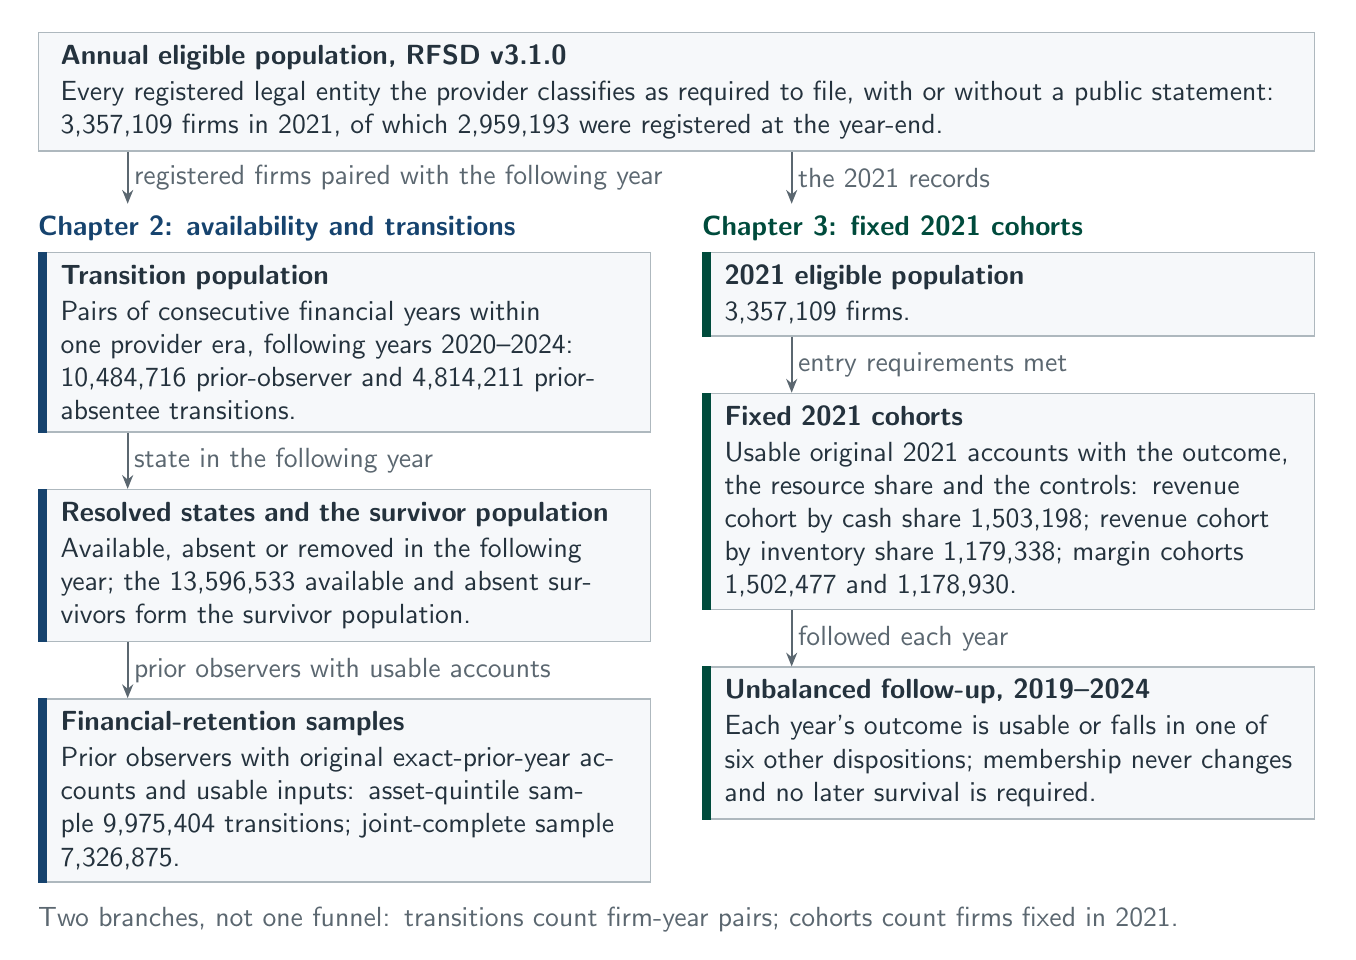
\begin{tikzpicture}[x=1in, y=1in]
\path (0,0) -- (6.5,0);
\node[top] (N0) at (0.05,-0.02) {\textbf{Annual eligible population, RFSD v3.1.0}\\[1pt]Every registered legal entity the provider classifies as required to file, with or without a public statement: 3,357,109 firms in 2021, of which 2,959,193 were registered at the year-end.};
\node[col] (L1) at ([yshift=-0.50in]N0.south west) {\textbf{Transition population}\\[1pt]Pairs of consecutive financial years within one provider era, following years 2020--2024: 10,484,716 prior-observer and 4,814,211 prior-absentee transitions.};
\node[col] (L2) at ([yshift=-0.28in]L1.south west) {\textbf{Resolved states and the survivor population}\\[1pt]Available, absent or removed in the following year; the 13,596,533 available and absent survivors form the survivor population.};
\node[col] (L3) at ([yshift=-0.28in]L2.south west) {\textbf{Financial-retention samples}\\[1pt]Prior observers with original exact-prior-year accounts and usable inputs: asset-quintile sample 9,975,404 transitions; joint-complete sample 7,326,875.};
\node[col, anchor=north east] (R1) at ([yshift=-0.50in]N0.south east) {\textbf{2021 eligible population}\\[1pt]3,357,109 firms.};
\node[col] (R2) at ([yshift=-0.28in]R1.south west) {\textbf{Fixed 2021 cohorts}\\[1pt]Usable original 2021 accounts with the outcome, the resource share and the controls: revenue cohort by cash share 1,503,198; revenue cohort by inventory share 1,179,338; margin cohorts 1,502,477 and 1,178,930.};
\node[col] (R3) at ([yshift=-0.28in]R2.south west) {\textbf{Unbalanced follow-up, 2019--2024}\\[1pt]Each year's outcome is usable or falls in one of six other dispositions; membership never changes and no later survival is required.};
\node[head, text=navy] at ([yshift=0.05in]L1.north west) {Chapter 2: availability and transitions};
\node[head, text=green] at ([yshift=0.05in]R1.north west) {Chapter 3: fixed 2021 cohorts};
\fill[navy] (L1.north west) rectangle ([xshift=3.2pt]L1.south west);
\fill[navy] (L2.north west) rectangle ([xshift=3.2pt]L2.south west);
\fill[navy] (L3.north west) rectangle ([xshift=3.2pt]L3.south west);
\fill[green] (R1.north west) rectangle ([xshift=3.2pt]R1.south west);
\fill[green] (R2.north west) rectangle ([xshift=3.2pt]R2.south west);
\fill[green] (R3.north west) rectangle ([xshift=3.2pt]R3.south west);
\coordinate (LX) at ([xshift=0.45in]L1.north west); \coordinate (RX) at ([xshift=0.45in]R1.north west);
\draw[arrow] (LX |- N0.south) -- ($(LX |- L1.north)+(0,0.24in)$) node[lab, pos=0.5] {registered firms paired with the following year};
\draw[arrow] (LX |- L1.south) -- (LX |- L2.north) node[lab, pos=0.5] {state in the following year};
\draw[arrow] (LX |- L2.south) -- (LX |- L3.north) node[lab, pos=0.5] {prior observers with usable accounts};
\draw[arrow] (RX |- N0.south) -- ($(RX |- R1.north)+(0,0.24in)$) node[lab, pos=0.5] {the 2021 records};
\draw[arrow] (RX |- R1.south) -- (RX |- R2.north) node[lab, pos=0.5] {entry requirements met};
\draw[arrow] (RX |- R2.south) -- (RX |- R3.north) node[lab, pos=0.5] {followed each year};
\path let \p1 = (L3.south), \p2 = (R3.south) in coordinate (B) at (0.05, {min(\y1, \y2)});
\node[anchor=north west, inner sep=0pt, text width=6.3in, align=left, text=muted] at ([yshift=-0.12in]B) {Two branches, not one funnel: transitions count firm-year pairs; cohorts count firms fixed in 2021.};
\end{tikzpicture}}
\pdfpagewidth=6.5in \pdfpageheight=\dimexpr\ht\flowbox+\dp\flowbox+0.08in\relax
\hoffset=-1in \voffset=-1in \topskip=0pt \parskip=0pt
\shipout\vbox to \pdfpageheight{\vskip0.04in\hbox to 6.5in{\usebox\flowbox\hss}\vss}
\csname @@end\endcsname
